\documentclass[11pt,]{article}
\usepackage[left=1in,top=1in,right=1in,bottom=1in]{geometry}
\newcommand*{\authorfont}{\fontfamily{phv}\selectfont}
\usepackage[]{mathpazo}


  \usepackage[T1]{fontenc}
  \usepackage[utf8]{inputenc}



\usepackage{abstract}
\renewcommand{\abstractname}{}    % clear the title
\renewcommand{\absnamepos}{empty} % originally center

\renewenvironment{abstract}
 {{%
    \setlength{\leftmargin}{0mm}
    \setlength{\rightmargin}{\leftmargin}%
  }%
  \relax}
 {\endlist}

\makeatletter
\def\@maketitle{%
  \newpage
%  \null
%  \vskip 2em%
%  \begin{center}%
  \let \footnote \thanks
    {\fontsize{18}{20}\selectfont\raggedright  \setlength{\parindent}{0pt} \@title \par}%
}
%\fi
\makeatother




\setcounter{secnumdepth}{3}


\usepackage{graphicx,grffile}
\makeatletter
\def\maxwidth{\ifdim\Gin@nat@width>\linewidth\linewidth\else\Gin@nat@width\fi}
\def\maxheight{\ifdim\Gin@nat@height>\textheight\textheight\else\Gin@nat@height\fi}
\makeatother
% Scale images if necessary, so that they will not overflow the page
% margins by default, and it is still possible to overwrite the defaults
% using explicit options in \includegraphics[width, height, ...]{}
\setkeys{Gin}{width=\maxwidth,height=\maxheight,keepaspectratio}

\title{Título\\
Subtítulo\\
Subtítulo  }



\author{\Large Darihana Linares Laureano\vspace{0.05in} \newline\normalsize\emph{Estudiante de Licenciatura en Geografía mención recursos naturales y
ecoturismo, Universidad Autónoma de Santo Domingo (UASD)}  }


\date{}

\usepackage{titlesec}

\titleformat*{\section}{\normalsize\bfseries}
\titleformat*{\subsection}{\normalsize\itshape}
\titleformat*{\subsubsection}{\normalsize\itshape}
\titleformat*{\paragraph}{\normalsize\itshape}
\titleformat*{\subparagraph}{\normalsize\itshape}

\titlespacing{\section}
{0pt}{36pt}{0pt}
\titlespacing{\subsection}
{0pt}{36pt}{0pt}
\titlespacing{\subsubsection}
{0pt}{36pt}{0pt}





\newtheorem{hypothesis}{Hypothesis}
\usepackage{setspace}

\makeatletter
\@ifpackageloaded{hyperref}{}{%
\ifxetex
  \PassOptionsToPackage{hyphens}{url}\usepackage[setpagesize=false, % page size defined by xetex
              unicode=false, % unicode breaks when used with xetex
              xetex]{hyperref}
\else
  \PassOptionsToPackage{hyphens}{url}\usepackage[unicode=true]{hyperref}
\fi
}

\@ifpackageloaded{color}{
    \PassOptionsToPackage{usenames,dvipsnames}{color}
}{%
    \usepackage[usenames,dvipsnames]{color}
}
\makeatother
\hypersetup{breaklinks=true,
            bookmarks=true,
            pdfauthor={Darihana Linares Laureano (Estudiante de Licenciatura en Geografía mención recursos naturales y
ecoturismo, Universidad Autónoma de Santo Domingo (UASD))},
             pdfkeywords = {palabra clave 1, palabra clave 2},  
            pdftitle={Título\\
Subtítulo\\
Subtítulo},
            colorlinks=true,
            citecolor=blue,
            urlcolor=blue,
            linkcolor=magenta,
            pdfborder={0 0 0}}
\urlstyle{same}  % don't use monospace font for urls

% set default figure placement to htbp
\makeatletter
\def\fps@figure{htbp}
\makeatother

\usepackage{pdflscape} \newcommand{\blandscape}{\begin{landscape}}
\newcommand{\elandscape}{\end{landscape}} \usepackage{float}
\floatplacement{figure}{H}
\newcommand{\beginsupplement}{ \setcounter{table}{0} \renewcommand{\thetable}{S\arabic{table}} \setcounter{figure}{0} \renewcommand{\thefigure}{S\arabic{figure}} }


% add tightlist ----------
\providecommand{\tightlist}{%
\setlength{\itemsep}{0pt}\setlength{\parskip}{0pt}}

\begin{document}
	
% \pagenumbering{arabic}% resets `page` counter to 1 
%
% \maketitle

{% \usefont{T1}{pnc}{m}{n}
\setlength{\parindent}{0pt}
\thispagestyle{plain}
{\fontsize{18}{20}\selectfont\raggedright 
\maketitle  % title \par  

}

{
   \vskip 13.5pt\relax \normalsize\fontsize{11}{12} 
\textbf{\authorfont Darihana Linares Laureano} \hskip 15pt \emph{\small Estudiante de Licenciatura en Geografía mención recursos naturales y
ecoturismo, Universidad Autónoma de Santo Domingo (UASD)}   

}

}








\begin{abstract}

    \hbox{\vrule height .2pt width 39.14pc}

    \vskip 8.5pt % \small 

\noindent Resumen del manuscrito


\vskip 8.5pt \noindent \emph{Keywords}: palabra clave 1, palabra clave 2 \par

    \hbox{\vrule height .2pt width 39.14pc}



\end{abstract}


\vskip 6.5pt


\noindent  \section{Introducción}\label{introducciuxf3n}

Desde mediados del siglo XVII es posible visualizar el interés del
hombre a estudiar la flora, la fauna y el medio en el que están en
conjunto con las interacciones que se producen entre ellos, pero no es
hasta mediados del siglo XIX cuando se introduce el término Ecología y
su definición, que se empieza a englobar en este tipo de estudios en una
categoría (De la Llata Loyola, 2003). A partir de este punto se
reconocieron distintos campos de estudios y se implementaron nuevos
métodos de análisis, entre los cuales destacan la ecología numérica y
métodos como el análisis multivariático. Según P. Legendre \& Legendre
(2012), la ecología numérica no es más que una de las disciplinas de la
ecología cuantitativa, la cual a la vez es una de las divisiones de la
ecología matemática.

La ecología numérica se concentra en el estudio y análisis de conjuntos
de datos ecológicos, a fin de poder detallar y comprender la
configuración de los conjuntos de datos, combinando diversas
perspectivas numéricas y disciplinas, procedentes de la Geografía, las
matemáticas físicas, taxonomía numérica, parámetros estadísticos y otros
más (P. Legendre \& Legendre, 2012). El análisis de conjuntos de datos
ecológicos, especialmente de la flora, resulta importante tanto para la
ciencia, como para la economía o el sector de salud, por eso se han
establecido distintas parcelas permanentes de medición y monitoreo
forestal donde se colectan datos sobre la diversidad forestal, su
estructura, el crecimiento y su productividad (Pineda, 2014). En el
estudio de las plantas a través de la Ecología Numérica se usan diversas
técnicas que permiten obtener información sobre el rango de asociación,
agrupamiento, ordenamiento, diversidad, autocorrelación, etcétera,
diferentes herramientas para usar las técnicas.

La medición de la asociación es un coeficiente que sirve para medir y
asociar los datos de variables cualitativos y cuantitativos. La medición
de estas variables se puede hacer por dos modos el \emph{Q} y el
\emph{R}, el primero consiste en hacer una comparación de un dúo de
objetos y el segundo consiste en realizar una descripción de un par de
objetos y luego compararlos. Para el modo \emph{Q} se miden la
asociación según la similaridad o disimilaridad de un par de objetos.
Mientras que para el modo R se mide el grado de dependencia existente
entre las variables, entre los cuales se puede mencionar la covarianza o
el coeficiente de correlación (Borcard, Gillet, Legendre, \& others,
2011).

En cambio, el análisis de agrupamiento o clúster análisis es una técnica
que consiste en separar un conjunto de datos y luego estructurarlos, sin
dejar uno fuera de lugar, como subconjuntos con distintas categorías o
jerarquías de acuerdo a sus características. La finalidad de hacer un
agrupamiento es identificar los pequeños grupos dispersos en un espacio
discreto pero constante, este agrupamiento divide en conjunto de objetos
a estudiar, por lo que es necesario e importante que cada objeto
agrupado en otros subgrupos no se encuentre en otros (Borcard et al.,
2011).

En el caso del análisis de ordenamiento, son técnicas que consisten en
simplificar la magnitud de los datos. Todas estas técnicas muestran las
predisposiciones esenciales de variabilidad de cada dato que se
encuentran en un campo de dimensiones simplificadas, organizando los
ejes con rangos decreciente de varianza explicada en cada uno de los
ejes sucesivo, de forma convencional. Estos tipos de análisis pueden ser
tanto no restringido o simple, como restringido o canónico. En donde
para el primero, las tendencias o predisposiciones del grupo que
interesa no está restringida por otro grupo. Entre sus técnicas
principales de análisis están los de componentes principales
(\emph{PCA}) basado en un vector propio y se utiliza en datos
cuantitativos sin tratamiento preservando la distancia euclídea, los de
correspondencia (\emph{CA}) que se usa en datos frecuentes con
dimensiones uniformes y positivos, y los de coordenadas principales
(\emph{PCoA}) que se concentra en organizar las matrices de
disimilaridad, usualmente, con el modo \emph{Q} en vez de tablas de
sitio por variables (Borcard et al., 2011).

Mientras que, para el segundo análisis de ordenamiento, restringido o
canónico, a diferencia de la simple, es una técnica que relaciona dos o
más conjunto de datos en el proceso de organización u ordenación.
Algunas de sus técnicas principales son análisis de redundancia
(\emph{RDA}) que consiste en la combinación de la regresión y \emph{PCA}
que funciona como una extensión de diversos análisis que muestran la
respuesta multivariante de datos, y el análisis de correspondencia
canónica (\emph{CCA}) que funciona como un aproximado de una regresión
Gaussiana multivariante, además, este se caracteriza por organizar las
especies en todos los ejes canónicos acore a su configuración ecológica
óptima (Borcard et al., 2011).

En cuanto a la diversidad, según Borcard et al. (2011) y Magurran
(1988), esto alude a la variedad y cantidad de especies en un espacio
determinado, esta variedad también se produce a nivel de comunidad. La
diversidad puede La diversidad va desde la diversidad local, hasta
heterogeneidad espacial de esta diversidad. La diversidad de especies
considerada como un número único puede ser medida por la riqueza o la
rarificación de especies usando la notación q o por la presencia o
ausencia de los datos de esta. Según Whittaker (1972), el entendimiento
de la diversidad y los cambios que conllevan, asociados a la
configuración del relieve los componentes \emph{alpha}, \emph{beta} y
\emph{gamma} serian de mucha utilidad. Donde la primera se refiere a la
riqueza de las especies existentes en una comunidad determinada,
considerada homogénea. La segunda, se trata del rango de cambios que se
producen en la estructura de especies que están en diferentes
comunidades en un espacio. Y la última, se refiere a la riqueza de
especies de forma conjuntiva que hay en una comunidad y que integra un
espacio determinado.

La autocorrelación, según Borcard et al. (2011), forma parte de los
análisis espaciales aplicados a datos ecológicos, que se produce por
distintos procesos y que mide puntos cercanos para afirmar si estos
poseen valores similares o distintos, por lo que la correlación puede
ser una correlación positiva o negativa.

La \emph{Myrtaceae} son una familia de plantas de árboles y arbustos
bastante numerosas compuestas caracterizadas por ser leñosas. Esta
familia de plantas pertenece al orden de los \emph{Myrtales}, teniendo a
nivel mundial 129 géneros y aproximadamente 5330 especies (Perez \& R,
s.f.). De sus características físicas se destacan sus hojas simples y
opuestas, tienden a ser perennes por lo que resulta poco común ver
individuos caducifolios, sus flores son hermafroditas y comúnmente son
de color blanco con simetría radial, según la especie de esta familia
los frutos tienen forma de bayas o cápsulas secas. De esta familia el
género más conocido es el \emph{Eucalypto Eucalyptus} por sus
propiedades medicinales y su madera dura. Esta familia está distribuida
en todos los continentes, pero predominan en América, África y Oceanía,
en climas templados, tropicales y subtropicales. Muchos consideran que
la importancia de esta familia está en lo económico, como la producción
de frutas para venta de zumos y mermeladas, producción de madera,
producción de papel, de carbón, además de ser usadas en la industria
farmacéutica, se usa en la cosmetología y en la producción de especias
(Almeida, 2019; Britannica, 2016; Lorenzo-Cáceres, s.f.).

El estudio de la biodiversidad de la flora en especial de una especie
vegetal es importante, debido a que permite conocer sus características
propias, ecosistémicas, su distribución, su capacidad productiva, su
potencial de uso y aportes a los humanos como a su ecosistema. Por todo
lo anterior, es importante determinar el objetivo de este estudio, el
cual se fragmenta así: \emph{a)} identificar si los grupos de mi
familia, Myrtaceae, se organizan de forma discontinua y acorde a la
composición de las especies; \emph{b)} indagar si existe algún tipo de
patrón que sea o no sea consistente con alguna variable ambiental o
atributo; \emph{c)} determinar cuántas especies indicadoras hay o si hay
alguna con preferencia por ciertas condiciones ambientales o atributos;
\emph{d)} investigar, en un espacio bidimensional, si hay una tendencia
de ordenación visible de las especies de Myrtaceae; \emph{e)} conocer si
las tendencias de ordenación se asocian con las variables ambientales o
atributos; \emph{f)} determinar, de acuerdo a la estimación de riqueza,
si mi familia está bien representada, tomando como buena representación
un 85\%; \emph{g)} investigar si existe una alguna asociación entre la
diversidad Alpha y las variables ambientales o atributos y cuales son
estas; \emph{h)} conocer si hay algún tipo de contribución local o de
alguna especie a la diversidad Beta; \emph{i)} identificar si hay alguna
especie que presente algún patrón aglomerado, cuál es y si presenta
alguna asociación con las variables ambientales; \emph{j)} y determinar
si los modelos de distribución de especies (\emph{SDM}) predicen
adecuadamente las ocurrencias de las especies.

\subsection{Área de estudio}\label{uxe1rea-de-estudio}

El área usada para este estudio se encuentra en \emph{BCI} (Isla de
Barrio Colorado), que es una isla perteneciente a Panamá, la cual se
formó cuando las aguas del río Chagres fueron represadas para construir
el Canal de Panamá (ver figura \ref{fig:bci_map}). Es considerada como
una colina con una superficie de 1,500 hectáreas sobresaliente a 137 m
en el lago Gatún, y que está localizada entre los 9º 09' N y 79º 51' W.
Esta isla se caracteriza por sus suelos arcillosos con profundidades
entre los 50 cm y 1 m, y su clima es común de las tierras bajas
tropicales (Pérez et al., 2005). El área de estudio, específicamente, es
una parcela permanente forestal para su medición y monitoreo de 50
hectáreas, establecida en 1980 por Stephen Hubbell y Robin Foster, en el
bosque húmedo tropical de \emph{BCI} (Hubbell, Foster, \& Condit, 2005).

Los datos extraidos de las especies forestales de la parcela se
obtuvieron a tráves de multiples censos desde 1982 hasta 2015 (un total
de 8 censos), en los cuales se hicieron identificación, marcado y
monitoreo de los tallos leñosos individuales de más de 10 mm de diámetro
a altura del pecho. Durante los 35 años se censarón más de 350,000
árboles individuales (Hubbell et al., 2005).

\begin{figure}
\centering
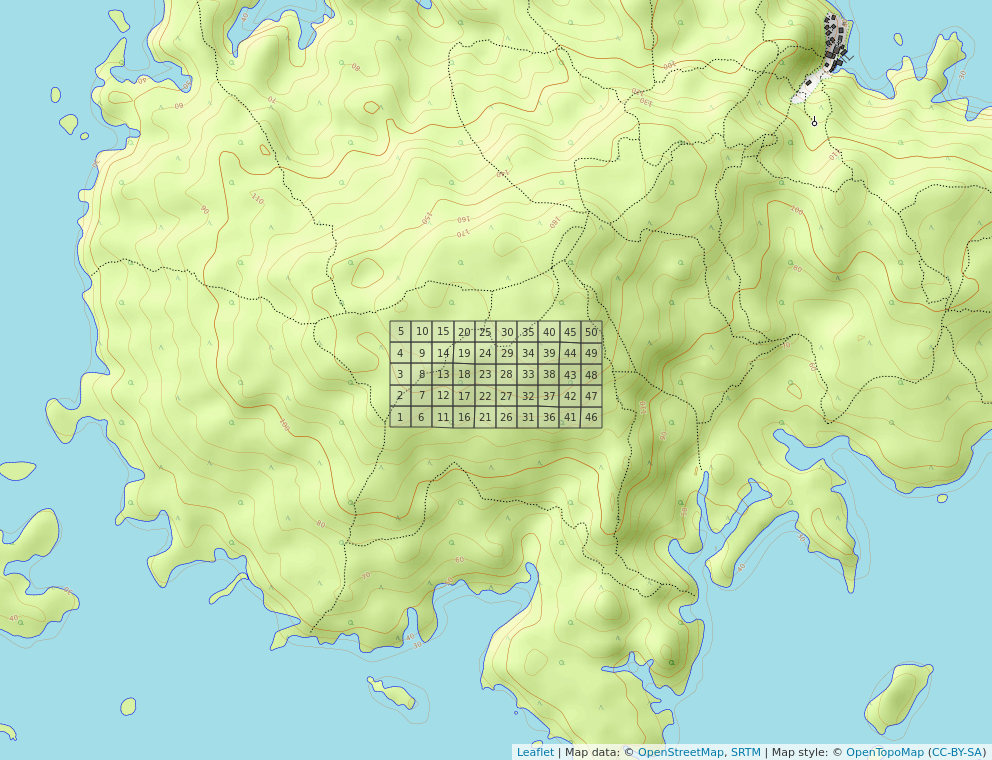
\includegraphics[width=1.00000\textwidth]{mapa_cuadros2.png}
\caption{Mapa de la Isla Barro Colorado y la parcela
permante\label{fig:bci_map}}
\end{figure}

\section{Metodología y materiales}\label{metodologuxeda-y-materiales}

Para el estudio de la biodiversidead de la familia \emph{Myrtaceae} se
usaron los datos censales de las 50 parcelas forestales de \emph{BCI},
los cuales fueron tratados y procesados con distintos algoritmos y
técnicas de medición, cálculo, análisis e interpretación por medio del
entorno de desarrollo intregado y libre, \emph{RStudio} (R Core Team,
2020). En cuanto a los gráficos presentes se obtuvieron por medio
\emph{R}, usando paquetes y funciones (ver tabla).

\section{Resultados}\label{resultados}

Ver tabla \ref{tab:abun_sp} y figura \ref{fig:abun_sp_q}

\section{Discusión}\label{discusiuxf3n}

\section{Agradecimientos}\label{agradecimientos}

\section{Información de soporte}\label{informaciuxf3n-de-soporte}

\ldots

\section{\texorpdfstring{\emph{Script}
reproducible}{Script reproducible}}\label{script-reproducible}

\ldots

\section*{Referencias}\label{referencias}
\addcontentsline{toc}{section}{Referencias}

\hypertarget{refs}{}
\hypertarget{ref-sandra2019myrtaceae}{}
Almeida, S. (2019). \emph{Myrtaceae, familia}. Retrieved from
\url{https://knoow.net/es/ciencias-tierra-vida/biologia-es/myrtaceae-familia/}

\hypertarget{ref-borcard2011numerical}{}
Borcard, D., Gillet, F., Legendre, P., \& others. (2011).
\emph{Numerical ecology with r} (Vol. 2). Springer.

\hypertarget{ref-encymyrtaceae}{}
Britannica, E. (2016). \emph{Myrtaceae}. Retrieved from
\url{https://www.britannica.com/plant/Myrtaceae}

\hypertarget{ref-de2003ecologia}{}
De la Llata Loyola, M. D. (2003). \emph{Ecología y medio ambiente}.
Editorial Progreso.

\hypertarget{ref-Hubbell2005barro}{}
Hubbell, S., Foster, R., \& Condit, R. (2005). \emph{Barro colorado
forest census plot data}. Retrieved from
\url{http://ctfs.si.edu/webatlas/datasets/bci/}

\hypertarget{ref-legendre2012numerical}{}
Legendre, P., \& Legendre, L. (2012). \emph{Numerical ecology}.
Elsevier.

\hypertarget{ref-josemyrtaceae}{}
Lorenzo-Cáceres, J. M. S. de. (s.f.). \emph{Familia myrtaceae}.
Retrieved from \url{https://www.arbolesornamentales.es/Myrtaceae.htm}

\hypertarget{ref-magurran1988ecological}{}
Magurran, A. E. (1988). \emph{Ecological diversity and its measurement}.
Princeton university press.

\hypertarget{ref-pereztree}{}
Perez, R., \& R, C. (s.f.). \emph{Tree atlas of panama}. Retrieved from
\url{http://ctfs.si.edu/PanamaAtlas/famdescr.php?Family=Myrtaceae}

\hypertarget{ref-perez2005metodologia}{}
Pérez, R., Aguilar, S., Condit, R., Foster, R., Hubbell, S., \& Lao, S.
(2005). Metodologia empleada en los censos de la parcela de 50 hectareas
de la isla de barro colorado, panamá. \emph{Centro de Ciencias
Forestales Del Tropico (CTFS) Y Instituto Smithsonian de Investigaciones
Tropicales (STRI)}, 1--24.

\hypertarget{ref-pineda2014analisis}{}
Pineda, P. (2014). \emph{Análisis del sistema de parcelas permanentes de
medición en los bosques de guatemala. informe final}. Guatemala:
Proyecto" Sistemas de información sobre la productividad de
los~\ldots{}.

\hypertarget{ref-R2020ALanguage}{}
R Core Team. (2020). \emph{R: A language and environment for statistical
computing}. Retrieved from \url{https://www.R-project.org/}

\hypertarget{ref-whittaker1972evolution}{}
Whittaker, R. H. (1972). Evolution and measurement of species diversity.
\emph{Taxon}, \emph{21}(2-3), 213--251.




\newpage
\singlespacing 
\end{document}
